% Звіт
% • Титульна сторінка
% • Опис хромосоми
% • Опис обраних варіантів схрещування та мутації
% • Опис головних гіперпараметрів та їх значення (розмір популяції, елітизм, ...) для кожного експерименту, графічні результати
% • Опис експериментів для кожної функції
% • Висновки
% • До звіту бажано додати (окремим файлом) анімаційне зображення процесу пошуку.

\documentclass{article}
\usepackage{graphicx}
\usepackage{epstopdf}
\usepackage{lipsum}
\usepackage[T2A]{fontenc}
\usepackage[utf8]{inputenc}

\graphicspath{ {../Images/} }

\epstopdfDeclareGraphicsRule{.gif}{png}{.png}{convert gif:#1 png:\OutputFile}
\AppendGraphicsExtensions{.gif}

\begin{document}
    \begin{titlepage}
        \begin{center}
        $\newline$
        \vspace{3.3cm}
        
        {\LARGE\textbf{Лабораторна робота №2\\"Реалізація алгоритму оптимізації роєм часток для пошуку глобального мінімуму функції."}}
        \vspace{10cm}
        \begin{flushright}
            \textbf{Роботу виконав:}\\Климентьєв Максим \\3-го курсу\\групи ФІ-21
        \end{flushright}
        \end{center}
    \end{titlepage}
    \newpage

    \tableofcontents

    \section{Опис головних гіперпараметрів та їх значення (розмір популяції, елітизм, ...) для кожного експерименту, графічні результати}
        \textbf{Розмір популяції} --- Просто кількість частинок
        \textbf{Кількість ітерацій} --- Просто кількість ітерацій
        \textbf{Швидкість руху} --- обмеження в швидкості для частинок

    \section{Опис експериментів для кожної функції}
        \textbf{Вони були однакові} --- Для кожної функції було проведено по 3 експерименти:
        \begin{enumerate}
            \item Коли кількість частинок велика
            \item Коли кількість ітерацій велика
            \item Коли швидкість руху велика
        \end{enumerate}

    \newpage
    \section{Опис результатів експериментів}
        \textbf{Ackley} --- має мінімум в точці 0
            \newline
            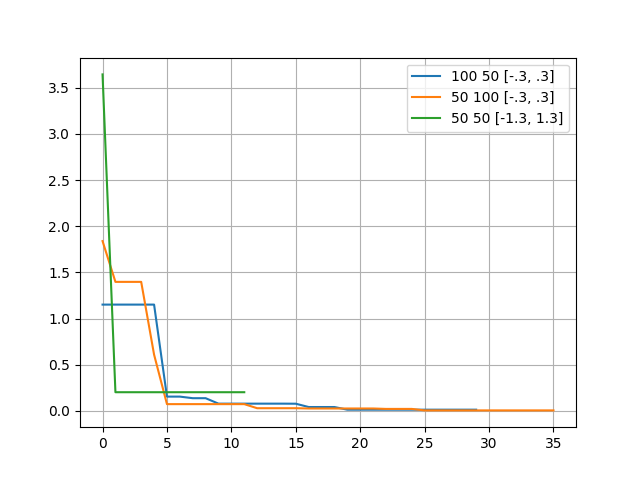
\includegraphics[scale=0.7]{Ackley_dif.png}
            \newline
            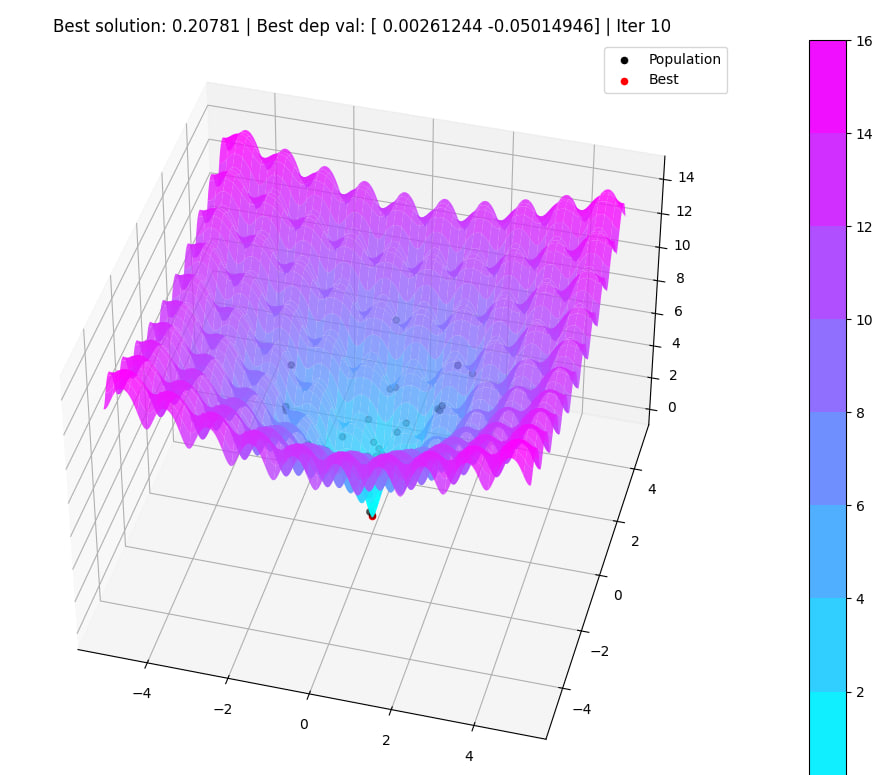
\includegraphics[scale=0.7]{Ackley.jpg}
            \newline
            % 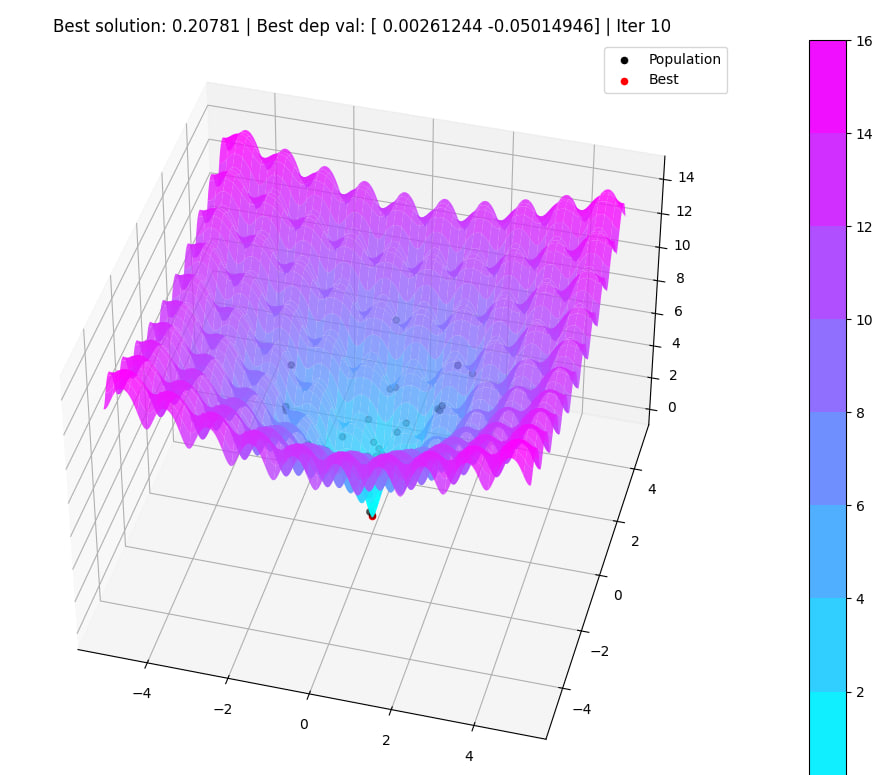
\includegraphics[scale=0.4]{Ackley.gif}
            
        \newpage
        \textbf{Rozenbrock} --- має мінімум в точці 0
            \newline
            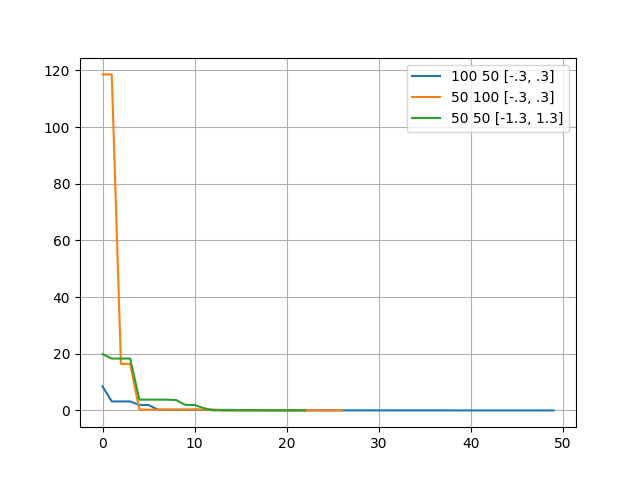
\includegraphics[scale=0.7]{Rozenbrock_dif.png}
            \newline
            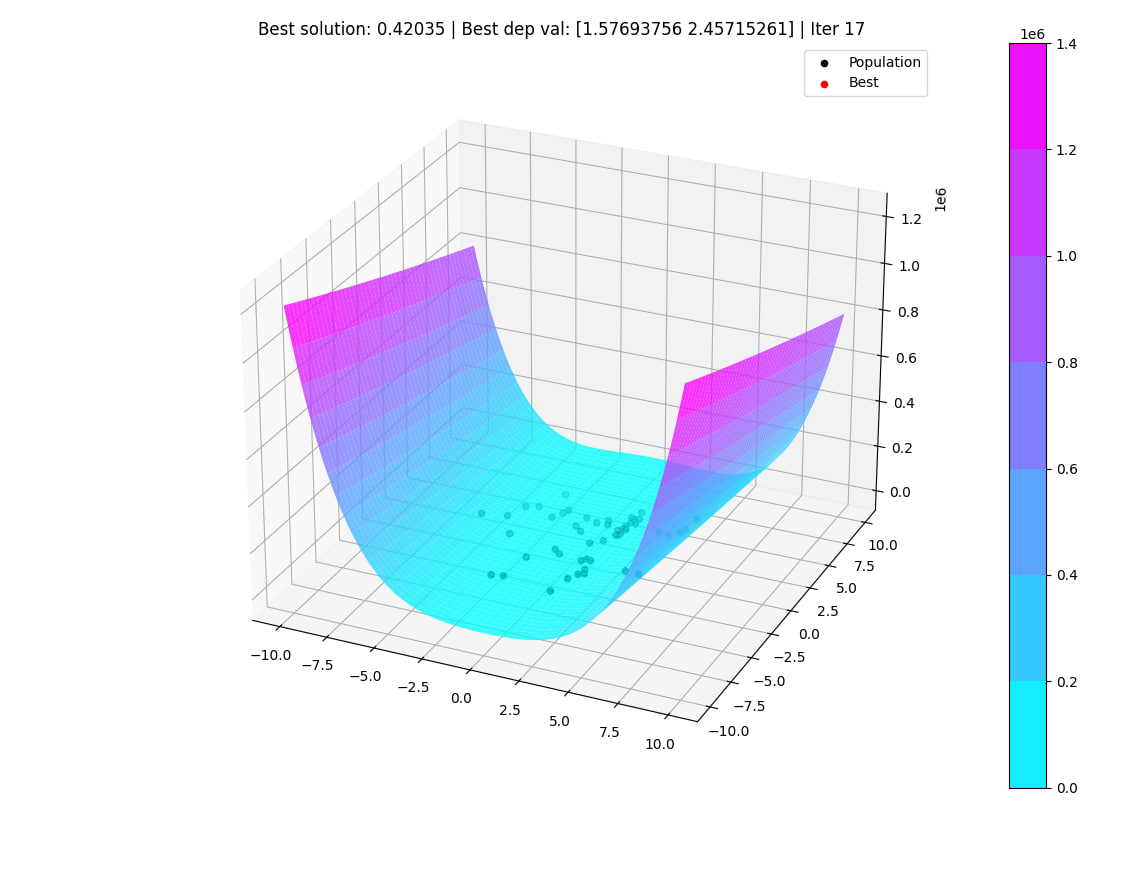
\includegraphics[scale=0.7]{Rozenbrock.jpg}
            \newline
            % 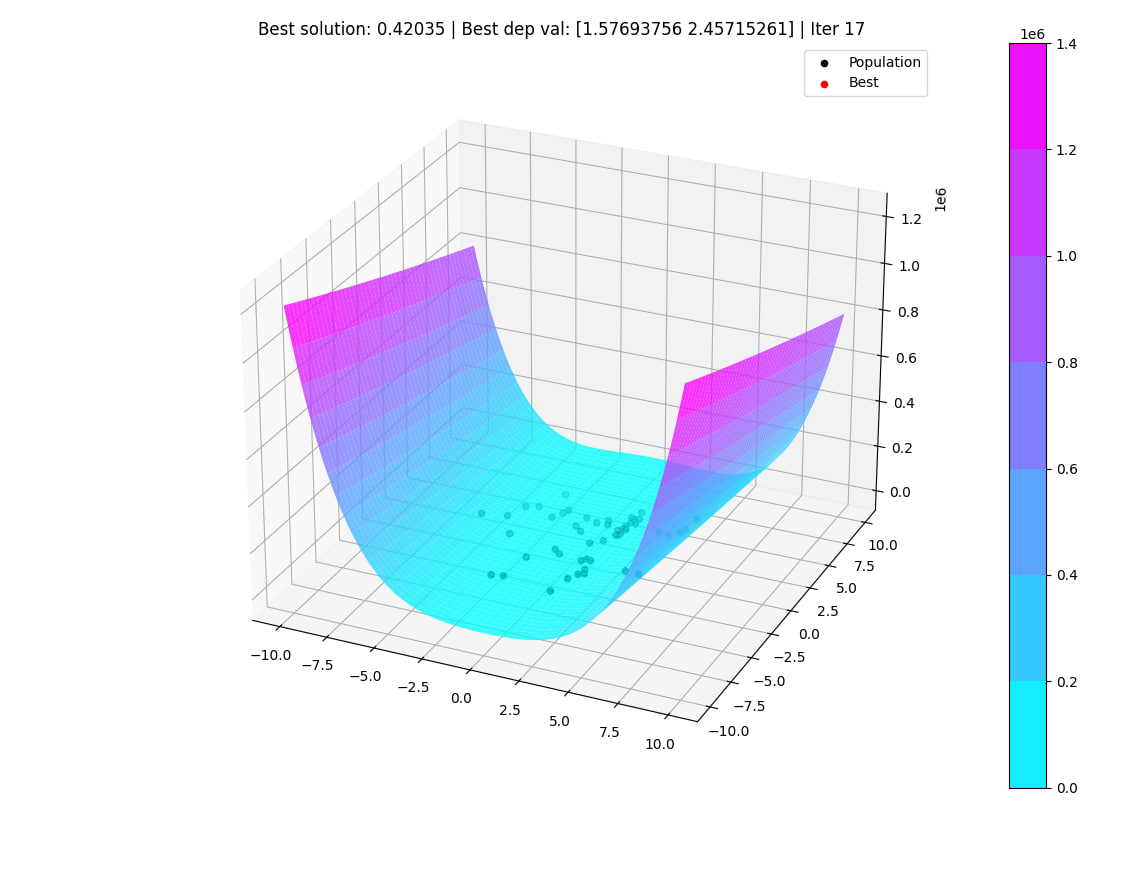
\includegraphics[scale=0.4]{Rozenbrock.gif}

        \newpage
        \textbf{CrossInTray} --- має мінімум в точці -2.06261
            \newline
            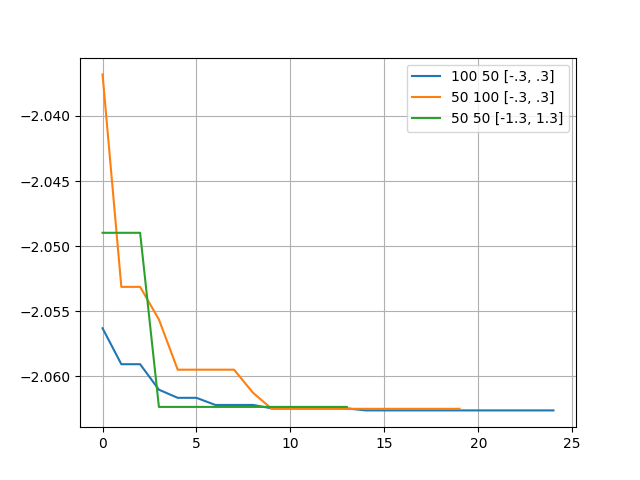
\includegraphics[scale=0.7]{CrossInTray_dif.png}
            \newline
            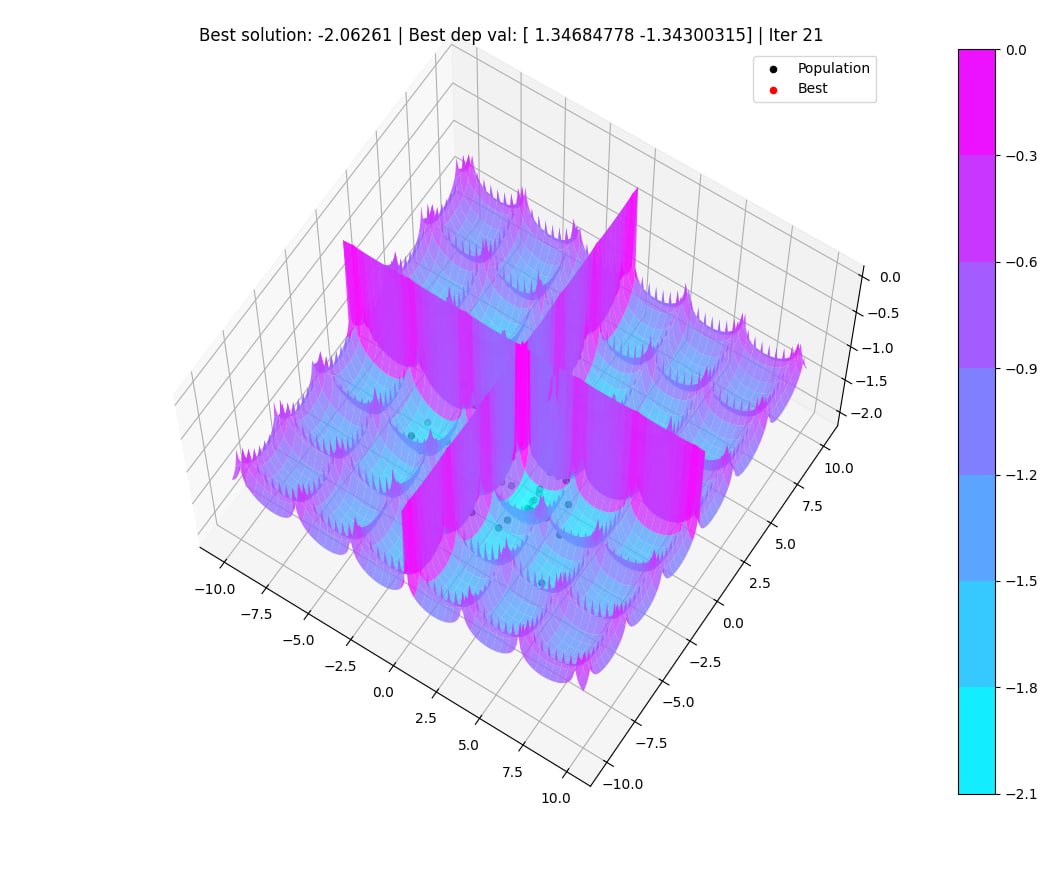
\includegraphics[scale=0.7]{CrossInTray.jpg}
            \newline
            % 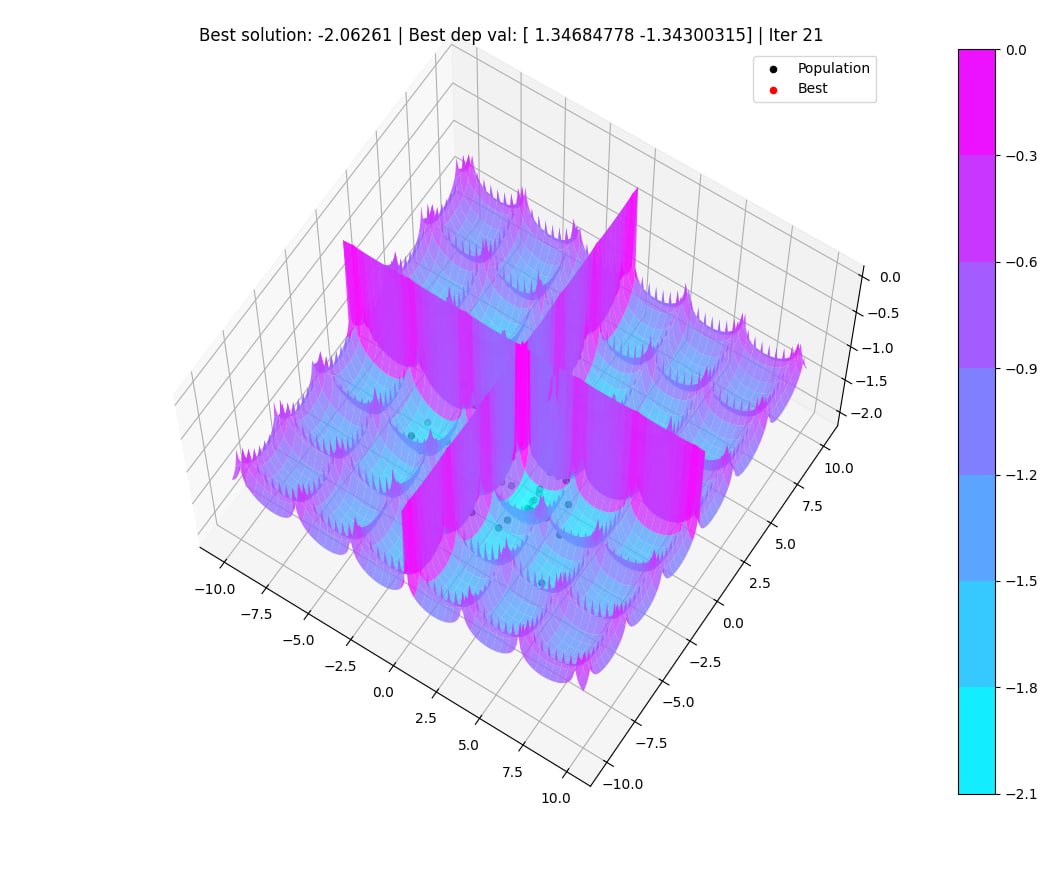
\includegraphics[scale=0.4]{CrossInTray.gif}

        \newpage
        \textbf{Holder} --- має мінімум в точці -19.2085
            \newline
            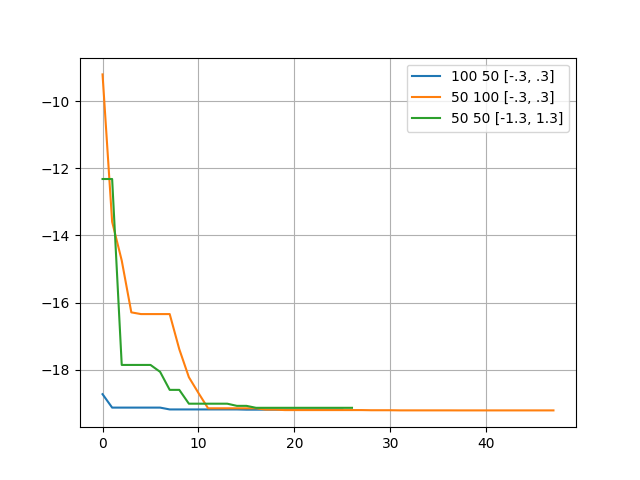
\includegraphics[scale=0.7]{Holder_dif.png}
            \newline
            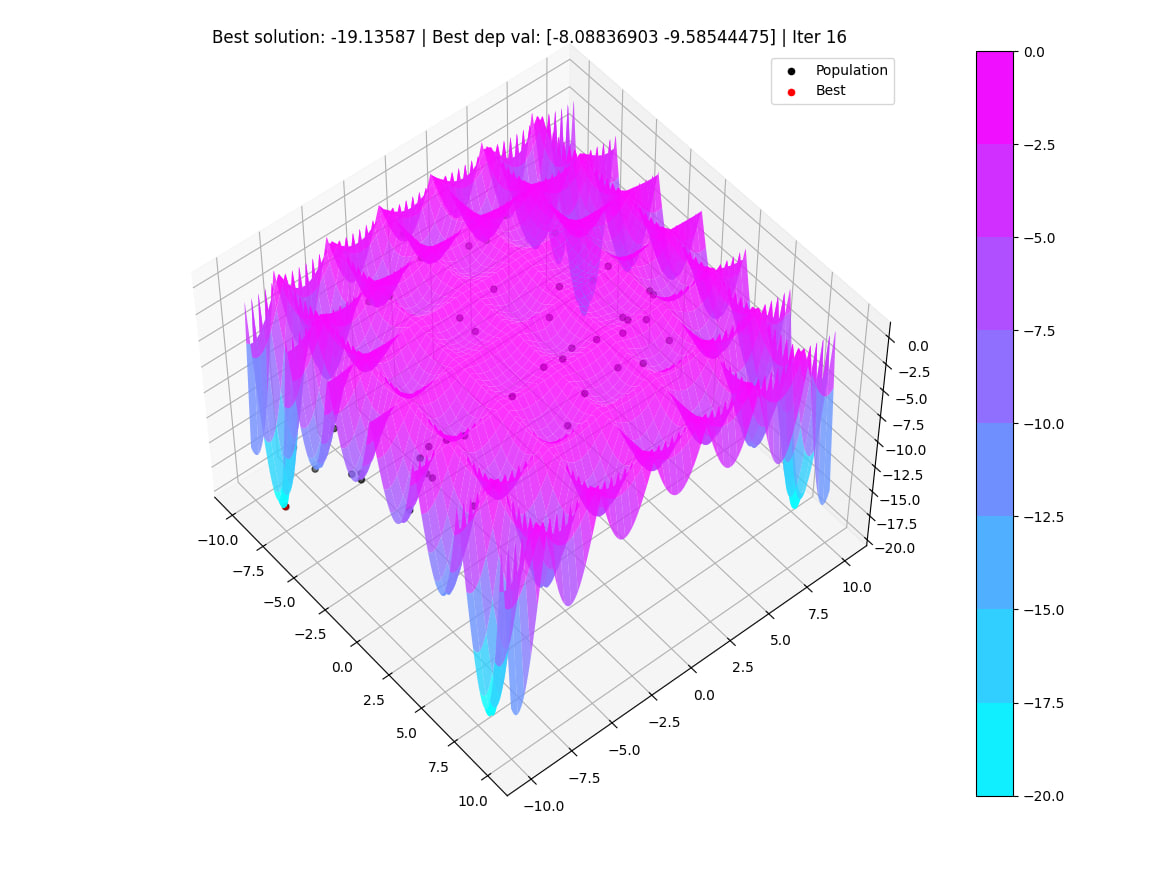
\includegraphics[scale=0.7]{Holder.jpg}
            \newline
            % 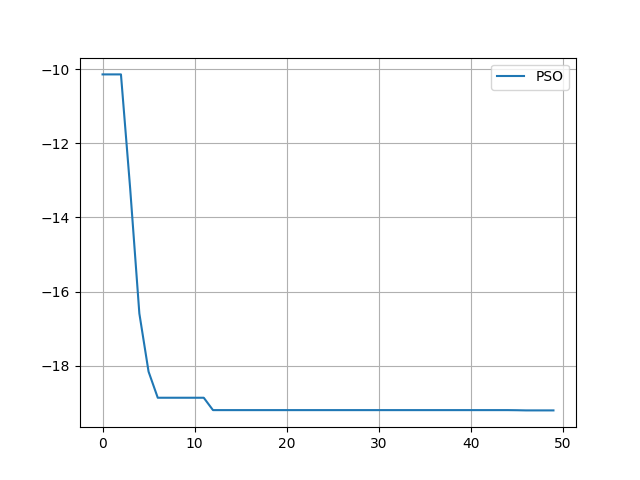
\includegraphics[scale=0.4]{Holder.gif}

        \newpage
        \textbf{McCormick} --- має мінімум в точці -1.9133
            \newline
            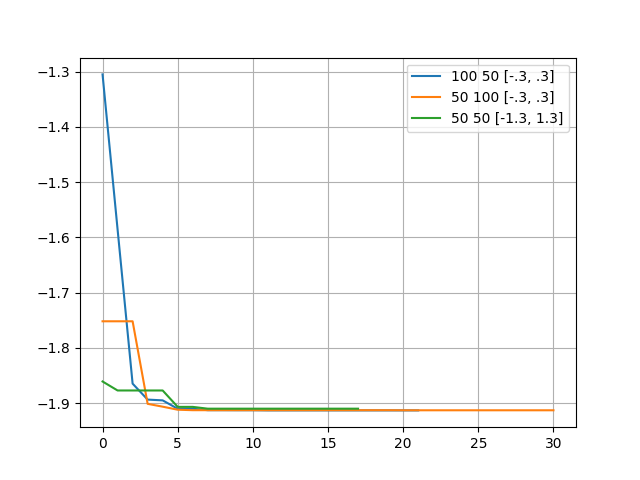
\includegraphics[scale=0.7]{McCormick_dif.png}
            \newline
            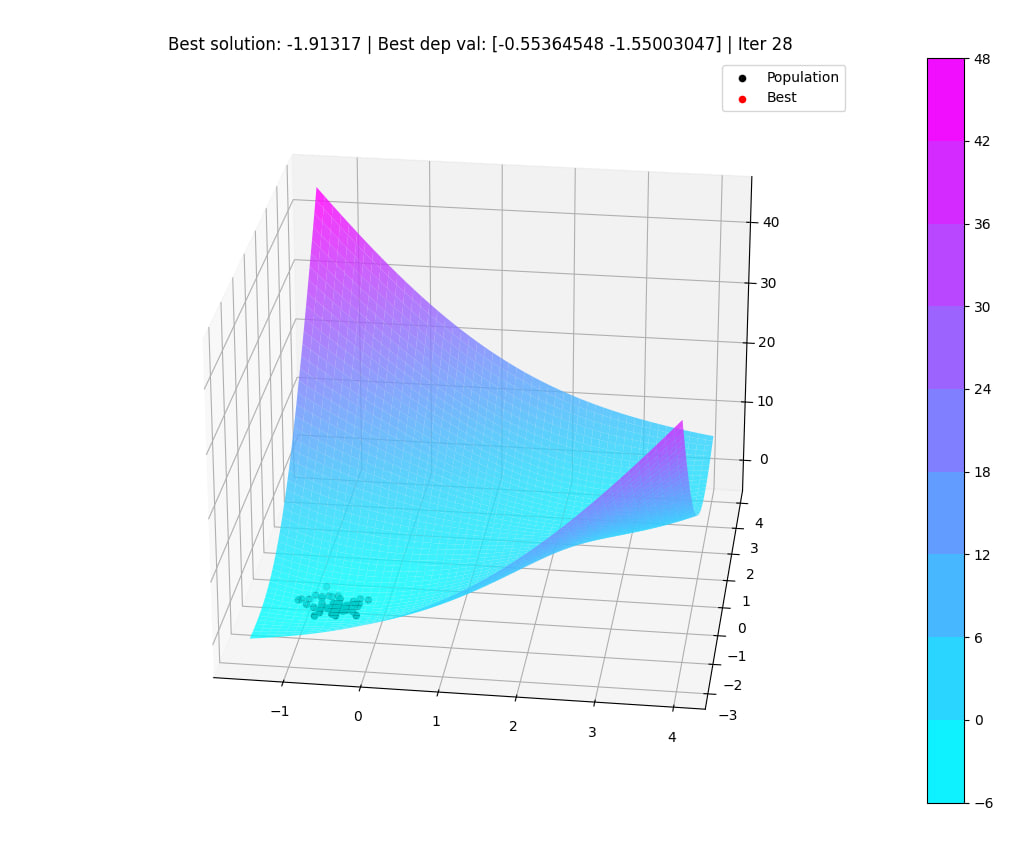
\includegraphics[scale=0.7]{McCormick.jpg}
            \newline
            % 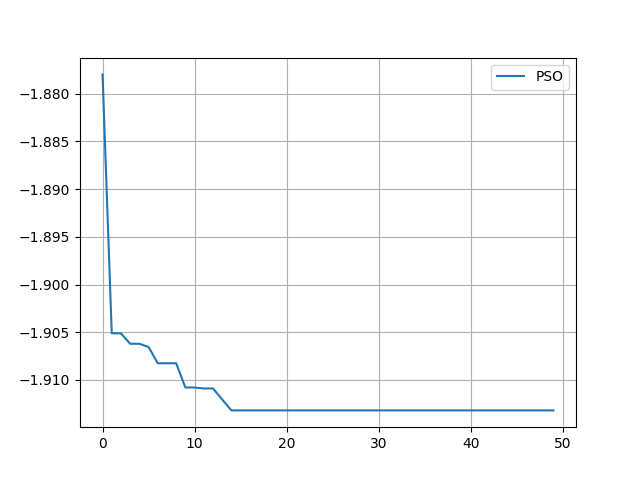
\includegraphics[scale=0.4]{McCormick.gif}

        \newpage
        \textbf{StyblinskiTang} --- має мінімум в точці -39.1661...
            \newline
            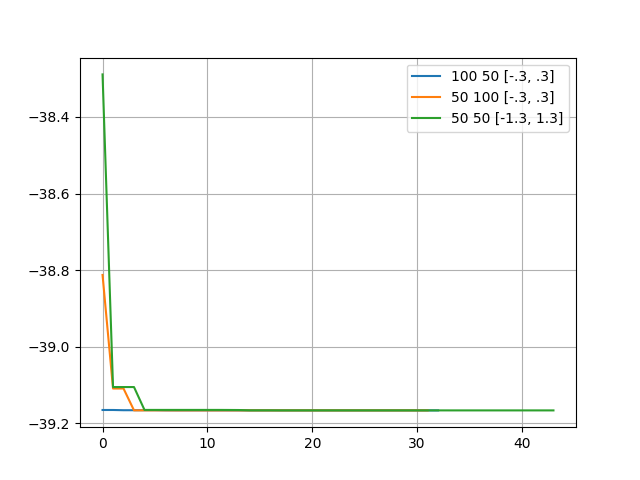
\includegraphics[scale=0.7]{StyblinskiTang_dif.png}
            \newline
            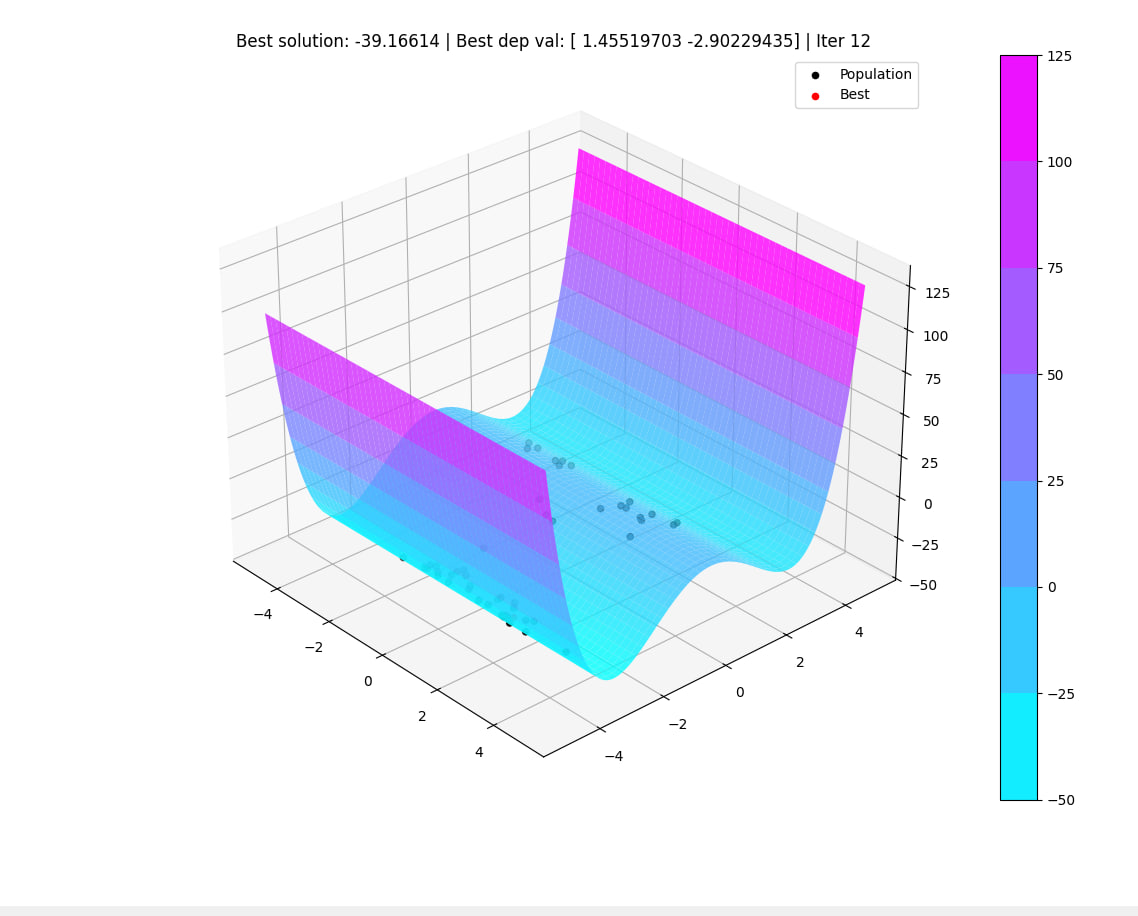
\includegraphics[scale=0.7]{StyblinskiTang.jpg}
            \newline
            % 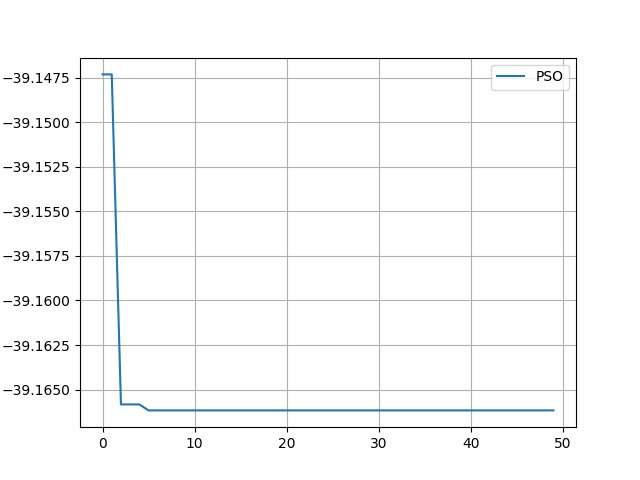
\includegraphics[scale=0.4]{StyblinskiTang.gif}

        \newpage
        \textbf{Reductor} --- шукаємо мінімальну вагу
            \newline
            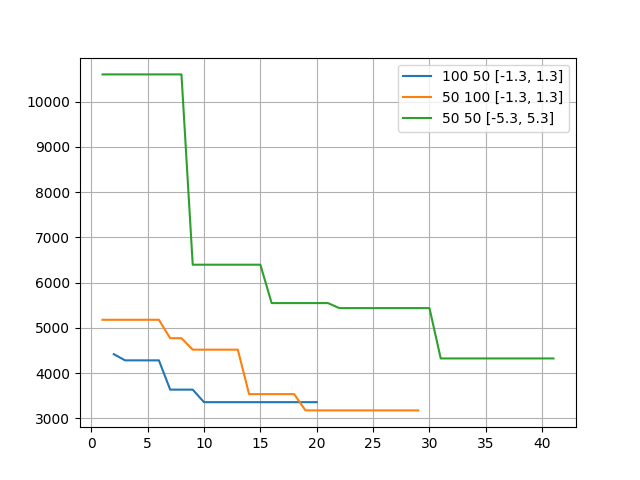
\includegraphics[scale=0.7]{Reductor_dif.png}
            \newline
    \newpage
    \section{Висновки}
        \textbf{Велика кількість популяції зазвичай краща}, ніж кількість ітерацій чи швидкість
        \newline
        \textbf{Велика кількість ітерацій або швидкість зазвичай гірше}, але швидкість інколи допомагає знайти результат, головне не переборщити.

\end{document}